\documentclass[a4paper,fontsize=12pt]{scrartcl}
\usepackage{tikz}
\begin{document}
\section*{Aoife Citizen}
\subsection*{matrix}
$$ C=\left(\begin{array}{cccc}
0.0&0.14&0.29&0.43\\0.14&0.29&0.43&0.57\\0.29&0.43&0.57&0.71\\\end{array}\right)$$
\subsection*{test patterns}
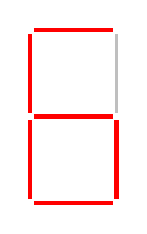
\begin{tikzpicture}
\draw[ultra thick,color=red](0,2.20)--(1,2.20);
\draw[ultra thick,color=red](-.05,1.15)--(-.05,2.15);
\draw[thick,color=lightgray](1.05,1.15)--(1.05,2.15);
\draw[ultra thick,color=red](0,1.10)--(1,1.10);
\draw[ultra thick,color=red](-.05,0.05)--(-.05,1.05);
\draw[ultra thick,color=red](1.05,0.05)--(1.05,1.05);
\draw[ultra thick,color=red](0,0)--(1,0);
\end{tikzpicture}
6
\qquad
 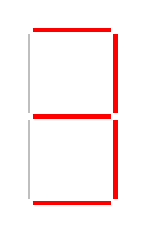
\begin{tikzpicture}
\draw[ultra thick,color=red](0,2.20)--(1,2.20);
\draw[thick,color=lightgray](-.05,1.15)--(-.05,2.15);
\draw[ultra thick,color=red](1.05,1.15)--(1.05,2.15);
\draw[ultra thick,color=red](0,1.10)--(1,1.10);
\draw[thick,color=lightgray](-.05,0.05)--(-.05,1.05);
\draw[ultra thick,color=red](1.05,0.05)--(1.05,1.05);
\draw[ultra thick,color=red](0,0)--(1,0);
\end{tikzpicture}
3
\qquad
 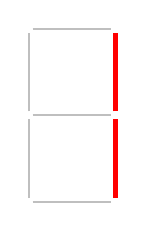
\begin{tikzpicture}
\draw[thick,color=lightgray](0,2.20)--(1,2.20);
\draw[thick,color=lightgray](-.05,1.15)--(-.05,2.15);
\draw[ultra thick,color=red](1.05,1.15)--(1.05,2.15);
\draw[thick,color=lightgray](0,1.10)--(1,1.10);
\draw[thick,color=lightgray](-.05,0.05)--(-.05,1.05);
\draw[ultra thick,color=red](1.05,0.05)--(1.05,1.05);
\draw[thick,color=lightgray](0,0)--(1,0);
\end{tikzpicture}
1
\subsection*{pretending to evolve the pattern}
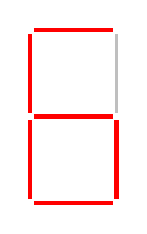
\begin{tikzpicture}
\draw[ultra thick,color=red](0,2.20)--(1,2.20);
\draw[ultra thick,color=red](-.05,1.15)--(-.05,2.15);
\draw[thick,color=lightgray](1.05,1.15)--(1.05,2.15);
\draw[ultra thick,color=red](0,1.10)--(1,1.10);
\draw[ultra thick,color=red](-.05,0.05)--(-.05,1.05);
\draw[ultra thick,color=red](1.05,0.05)--(1.05,1.05);
\draw[ultra thick,color=red](0,0)--(1,0);
\end{tikzpicture}
6
\qquad
 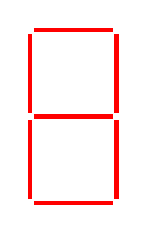
\begin{tikzpicture}
\draw[ultra thick,color=red](0,2.20)--(1,2.20);
\draw[ultra thick,color=red](-.05,1.15)--(-.05,2.15);
\draw[ultra thick,color=red](1.05,1.15)--(1.05,2.15);
\draw[ultra thick,color=red](0,1.10)--(1,1.10);
\draw[ultra thick,color=red](-.05,0.05)--(-.05,1.05);
\draw[ultra thick,color=red](1.05,0.05)--(1.05,1.05);
\draw[ultra thick,color=red](0,0)--(1,0);
\end{tikzpicture}
6
\qquad
 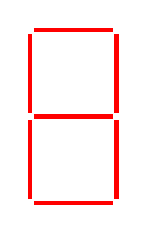
\begin{tikzpicture}
\draw[ultra thick,color=red](0,2.20)--(1,2.20);
\draw[ultra thick,color=red](-.05,1.15)--(-.05,2.15);
\draw[ultra thick,color=red](1.05,1.15)--(1.05,2.15);
\draw[ultra thick,color=red](0,1.10)--(1,1.10);
\draw[ultra thick,color=red](-.05,0.05)--(-.05,1.05);
\draw[ultra thick,color=red](1.05,0.05)--(1.05,1.05);
\draw[ultra thick,color=red](0,0)--(1,0);
\end{tikzpicture}
4
\qquad
 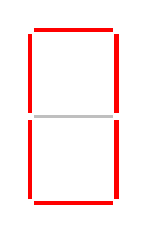
\begin{tikzpicture}
\draw[ultra thick,color=red](0,2.20)--(1,2.20);
\draw[ultra thick,color=red](-.05,1.15)--(-.05,2.15);
\draw[ultra thick,color=red](1.05,1.15)--(1.05,2.15);
\draw[thick,color=lightgray](0,1.10)--(1,1.10);
\draw[ultra thick,color=red](-.05,0.05)--(-.05,1.05);
\draw[ultra thick,color=red](1.05,0.05)--(1.05,1.05);
\draw[ultra thick,color=red](0,0)--(1,0);
\end{tikzpicture}
4
\qquad
 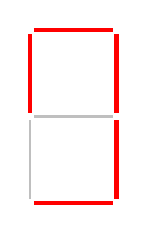
\begin{tikzpicture}
\draw[ultra thick,color=red](0,2.20)--(1,2.20);
\draw[ultra thick,color=red](-.05,1.15)--(-.05,2.15);
\draw[ultra thick,color=red](1.05,1.15)--(1.05,2.15);
\draw[thick,color=lightgray](0,1.10)--(1,1.10);
\draw[thick,color=lightgray](-.05,0.05)--(-.05,1.05);
\draw[ultra thick,color=red](1.05,0.05)--(1.05,1.05);
\draw[ultra thick,color=red](0,0)--(1,0);
\end{tikzpicture}
4
\qquad
 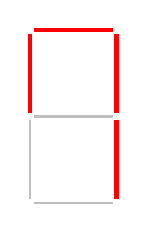
\begin{tikzpicture}
\draw[ultra thick,color=red](0,2.20)--(1,2.20);
\draw[ultra thick,color=red](-.05,1.15)--(-.05,2.15);
\draw[ultra thick,color=red](1.05,1.15)--(1.05,2.15);
\draw[thick,color=lightgray](0,1.10)--(1,1.10);
\draw[thick,color=lightgray](-.05,0.05)--(-.05,1.05);
\draw[ultra thick,color=red](1.05,0.05)--(1.05,1.05);
\draw[thick,color=lightgray](0,0)--(1,0);
\end{tikzpicture}
4
\qquad
 \\\\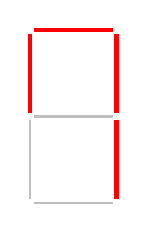
\begin{tikzpicture}
\draw[ultra thick,color=red](0,2.20)--(1,2.20);
\draw[ultra thick,color=red](-.05,1.15)--(-.05,2.15);
\draw[ultra thick,color=red](1.05,1.15)--(1.05,2.15);
\draw[thick,color=lightgray](0,1.10)--(1,1.10);
\draw[thick,color=lightgray](-.05,0.05)--(-.05,1.05);
\draw[ultra thick,color=red](1.05,0.05)--(1.05,1.05);
\draw[thick,color=lightgray](0,0)--(1,0);
\end{tikzpicture}
0
\qquad
 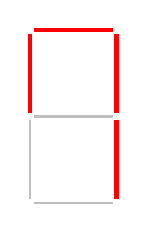
\begin{tikzpicture}
\draw[ultra thick,color=red](0,2.20)--(1,2.20);
\draw[ultra thick,color=red](-.05,1.15)--(-.05,2.15);
\draw[ultra thick,color=red](1.05,1.15)--(1.05,2.15);
\draw[thick,color=lightgray](0,1.10)--(1,1.10);
\draw[thick,color=lightgray](-.05,0.05)--(-.05,1.05);
\draw[ultra thick,color=red](1.05,0.05)--(1.05,1.05);
\draw[thick,color=lightgray](0,0)--(1,0);
\end{tikzpicture}
1
\qquad
 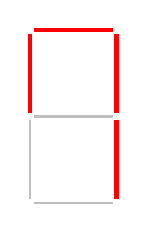
\begin{tikzpicture}
\draw[ultra thick,color=red](0,2.20)--(1,2.20);
\draw[ultra thick,color=red](-.05,1.15)--(-.05,2.15);
\draw[ultra thick,color=red](1.05,1.15)--(1.05,2.15);
\draw[thick,color=lightgray](0,1.10)--(1,1.10);
\draw[thick,color=lightgray](-.05,0.05)--(-.05,1.05);
\draw[ultra thick,color=red](1.05,0.05)--(1.05,1.05);
\draw[thick,color=lightgray](0,0)--(1,0);
\end{tikzpicture}
3
\qquad
 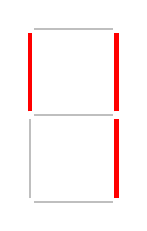
\begin{tikzpicture}
\draw[thick,color=lightgray](0,2.20)--(1,2.20);
\draw[ultra thick,color=red](-.05,1.15)--(-.05,2.15);
\draw[ultra thick,color=red](1.05,1.15)--(1.05,2.15);
\draw[thick,color=lightgray](0,1.10)--(1,1.10);
\draw[thick,color=lightgray](-.05,0.05)--(-.05,1.05);
\draw[ultra thick,color=red](1.05,0.05)--(1.05,1.05);
\draw[thick,color=lightgray](0,0)--(1,0);
\end{tikzpicture}
3
\qquad
 \subsection*{pretending to evolve the pattern with energies}
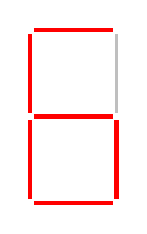
\begin{tikzpicture}
\draw[ultra thick,color=red](0,2.20)--(1,2.20);
\draw[ultra thick,color=red](-.05,1.15)--(-.05,2.15);
\draw[thick,color=lightgray](1.05,1.15)--(1.05,2.15);
\draw[ultra thick,color=red](0,1.10)--(1,1.10);
\draw[ultra thick,color=red](-.05,0.05)--(-.05,1.05);
\draw[ultra thick,color=red](1.05,0.05)--(1.05,1.05);
\draw[ultra thick,color=red](0,0)--(1,0);
\end{tikzpicture}
6
 0.466 \qquad
 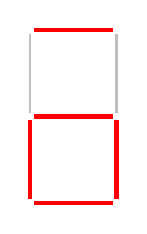
\begin{tikzpicture}
\draw[ultra thick,color=red](0,2.20)--(1,2.20);
\draw[thick,color=lightgray](-.05,1.15)--(-.05,2.15);
\draw[thick,color=lightgray](1.05,1.15)--(1.05,2.15);
\draw[ultra thick,color=red](0,1.10)--(1,1.10);
\draw[ultra thick,color=red](-.05,0.05)--(-.05,1.05);
\draw[ultra thick,color=red](1.05,0.05)--(1.05,1.05);
\draw[ultra thick,color=red](0,0)--(1,0);
\end{tikzpicture}
6
 0.095 \qquad
 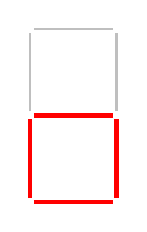
\begin{tikzpicture}
\draw[thick,color=lightgray](0,2.20)--(1,2.20);
\draw[thick,color=lightgray](-.05,1.15)--(-.05,2.15);
\draw[thick,color=lightgray](1.05,1.15)--(1.05,2.15);
\draw[ultra thick,color=red](0,1.10)--(1,1.10);
\draw[ultra thick,color=red](-.05,0.05)--(-.05,1.05);
\draw[ultra thick,color=red](1.05,0.05)--(1.05,1.05);
\draw[ultra thick,color=red](0,0)--(1,0);
\end{tikzpicture}
6
 0.932 \qquad
 \\\\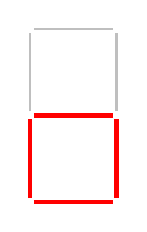
\begin{tikzpicture}
\draw[thick,color=lightgray](0,2.20)--(1,2.20);
\draw[thick,color=lightgray](-.05,1.15)--(-.05,2.15);
\draw[thick,color=lightgray](1.05,1.15)--(1.05,2.15);
\draw[ultra thick,color=red](0,1.10)--(1,1.10);
\draw[ultra thick,color=red](-.05,0.05)--(-.05,1.05);
\draw[ultra thick,color=red](1.05,0.05)--(1.05,1.05);
\draw[ultra thick,color=red](0,0)--(1,0);
\end{tikzpicture}
4
 0.276 \qquad
 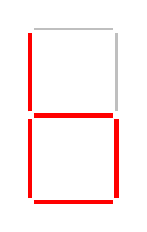
\begin{tikzpicture}
\draw[thick,color=lightgray](0,2.20)--(1,2.20);
\draw[ultra thick,color=red](-.05,1.15)--(-.05,2.15);
\draw[thick,color=lightgray](1.05,1.15)--(1.05,2.15);
\draw[ultra thick,color=red](0,1.10)--(1,1.10);
\draw[ultra thick,color=red](-.05,0.05)--(-.05,1.05);
\draw[ultra thick,color=red](1.05,0.05)--(1.05,1.05);
\draw[ultra thick,color=red](0,0)--(1,0);
\end{tikzpicture}
4
 0.393 \qquad
 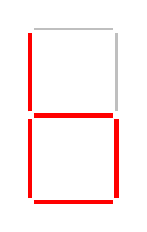
\begin{tikzpicture}
\draw[thick,color=lightgray](0,2.20)--(1,2.20);
\draw[ultra thick,color=red](-.05,1.15)--(-.05,2.15);
\draw[thick,color=lightgray](1.05,1.15)--(1.05,2.15);
\draw[ultra thick,color=red](0,1.10)--(1,1.10);
\draw[ultra thick,color=red](-.05,0.05)--(-.05,1.05);
\draw[ultra thick,color=red](1.05,0.05)--(1.05,1.05);
\draw[ultra thick,color=red](0,0)--(1,0);
\end{tikzpicture}
5
 0.127 \qquad
 \\\\\end{document}